\documentclass{article}
\usepackage{listings}
\usepackage{xcolor}
\usepackage{minted}
\usepackage{geometry}
\usepackage{float}
\usepackage{graphicx}
\usepackage{algorithm}
\usepackage{algpseudocode}
\usepackage{hyperref}
\usepackage{tabularx}

\geometry{
	textheight=9in,
	textwidth=6in,
	top=1in,
	headheight=12pt,
	headsep=25pt,
	footskip=30pt
}

\begin{document}
	
	\title{Selected Topics in Frontiers of Statistics First Assignment}
	\author{12111620 Yixuan Ding}
	\date{\today}
	\maketitle
	\section*{Graph Generation}
	As the question mentioned: First generate an undirected graph with 100 nodes,the smallest degree of each node is 2, the largest is 20. Also, the degree distribution of the graph is: $p(k) = k^{-2.5}$. After that, randomly select edges and turn them into directed edges, making the graph being directed.\\
	As for code implementation, first define a function named \textit{generate\_degree\_sequence} to generate a sequence of nodes whose degrees according with demand, then also define a function named \textit{generate\_directed\_graph} for final graph generation.\\
	The network visualization is shown as:
	\begin{figure}[H]
		\centering
		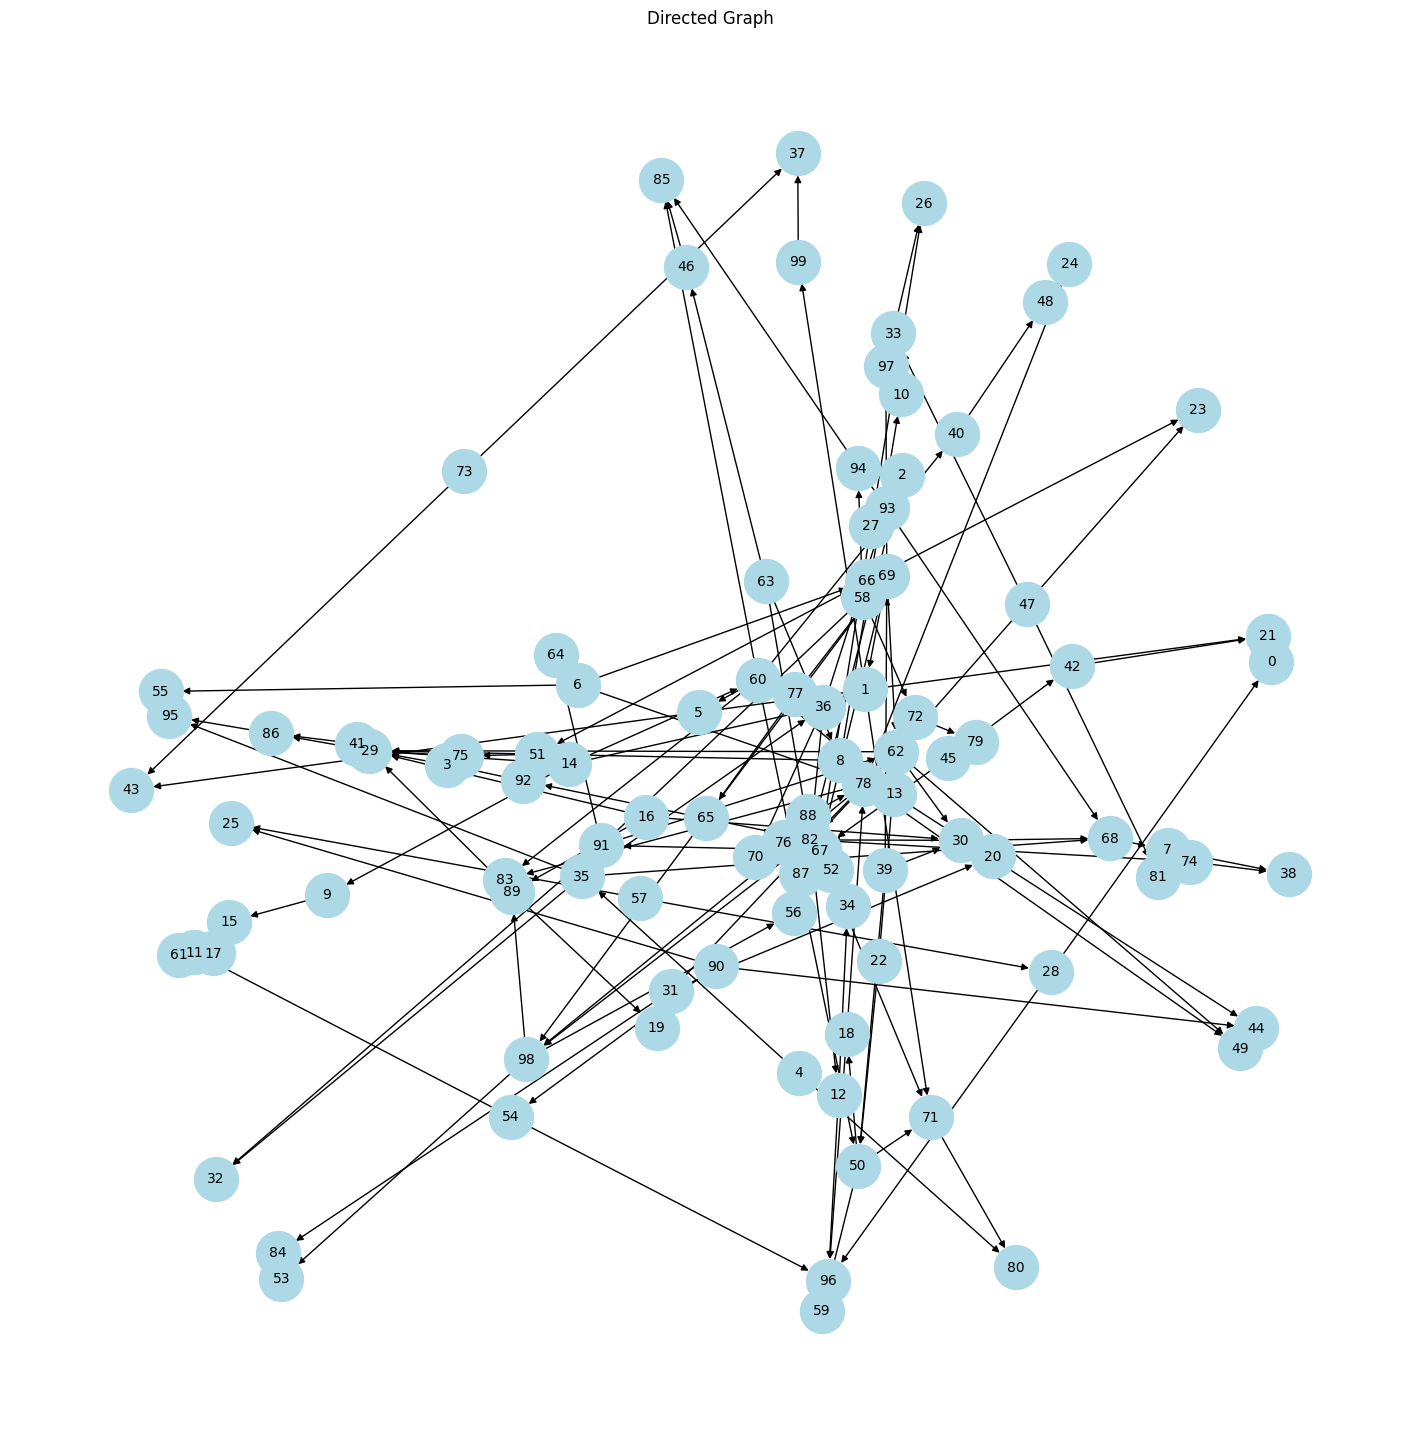
\includegraphics[scale=0.32]{network.png}
		\caption{Network Visualization}
	\end{figure}
	
	\section*{PageRank Algorithm Implementation}
	For the first problem, PageRank algorithm is implemented into graph generated before, with \\$\beta = 0.85$. Below is the implemented detail, which also define in the code script \textit{calculate\_pagerank}:\\
	
	\begin{algorithm}
		\caption{PageRank}\label{alg:pagerank}
		\begin{algorithmic}
			\State N $\gets $ Number of nodes in graph
			\State Initialize the pagerank of each node as $\frac{1}{N}$
			\For{\_ in range(max\_iterations)}
				\For{node in graph.nodes()}
					\State sum\_pr $\gets$ 0 
					\If{graph has neighbor}
						\For{node in graph's neighbors}
							\If{node's neighbor is null}
								\State Continue
							\EndIf
							\State sum\_pr += node's pagerank / number of node's neighbors
						
						\EndFor
					\Else
						\State sum\_pc $\gets$ 0
					\EndIf
				\State new pagerank of node $\gets$ (1-$\beta$)/N + $\beta$ * sum\_pr
				\EndFor
			\If{Converge}
				\State break
			\EndIf
			\State pagerank $\gets$ new\_pagerank
			\EndFor
		\end{algorithmic}
	\end{algorithm}
	
	\begin{figure}[H]
		\centering
		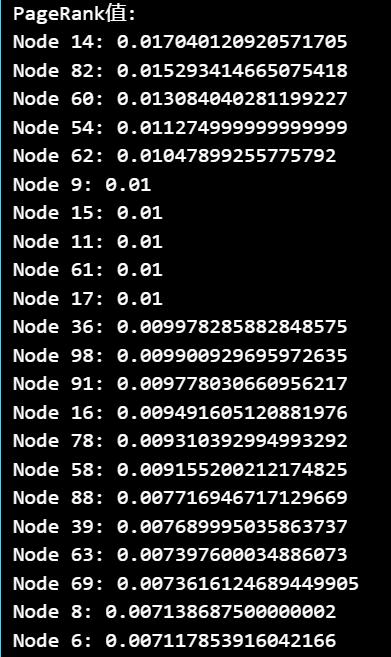
\includegraphics[scale=0.5]{pagerank.png}
		\caption{Part of Pagerank Outcome}
	\end{figure}
	
	Conduct the algorithm, then we can get the pagerank for each node, after that, discover the relationship of pagerank and degrees for nodes, which has a correlation coefficient of 0.503. The relationship is shown by the figure below:
	\begin{figure}[H]
		\centering
		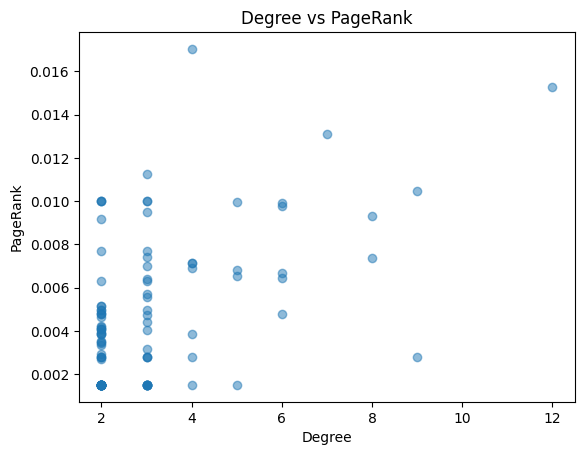
\includegraphics[scale=0.5]{relationship of pagerank and degree.png}
		\caption{Relationship of Pagerank and Degree of nodes}
	\end{figure}
	
	\section*{Spam Farm Design}
	Based on the graph generated before, design a spam farm to simulate an attack
	to the origin network to boosting the pagerank of the target page.
	The structure of spamfarm consists of three aspects:
	\begin{itemize}
		\item Accessible Nodes: Composed by the original node of directed graph, which represents the common webpage(harmless)
		\item Target Page: Page that we want to boost its pagerank by means of adding spam page
		\item Spam Pages: Harmful pages in the network, aiming for boosting pagerank of target page; need to be detected and removed.
	\end{itemize}
	\begin{figure}[H]
		\centering
		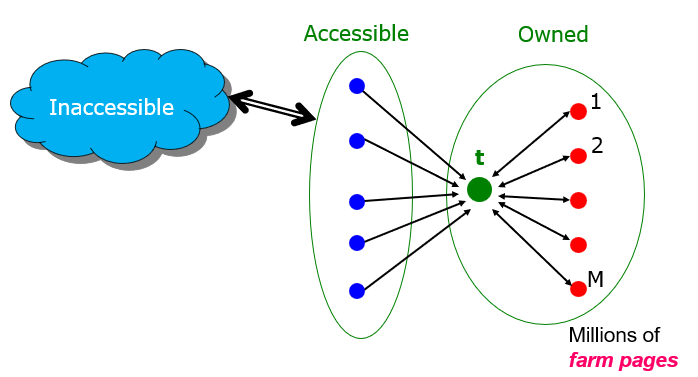
\includegraphics[scale=0.5]{spamfarm.png}
		\caption{Design of Spamfarm}
	\end{figure}
	
	To discover the relationship of target page's pagerank and the number of spam pages, a figure is shown below:
	\begin{figure}[H]
		\centering
		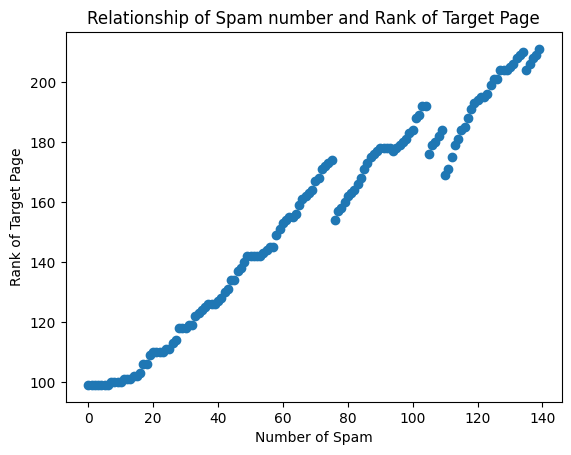
\includegraphics[scale=0.5]{Relationship of Spam Number and Pagerank of Target Page.png}
		\caption{Relationship of Spam Number and Pagerank of Target Page}
	\end{figure}
	It is easy to find that as the number of spam pages growing, the pagerank of target page will become higher.
	
	\section*{TrustRank Algorithm Implementation}
	In order to solve the spam farm situation, trustrank algorithm is introduced and implemented in the following report. Randomly, select 5\% percent of the accessible node to be trust node, according to which trustrank of each node is calculated and analyzed.
	
	\begin{algorithm}
		\caption{TrustRank}\label{alg:trustrank}
		\begin{algorithmic}
			\State seedsize $\gets$ 5\% amount of number of accessible nodes
			\State Trustvalue $\gets$ $\frac{1}{seedsize}$
			\State Initialize the $trustrank$ of each node \Comment{Randomly Select trust nodes from accessible nodes}
			\For{\_ in range(max\_iterations)}
			\For{node in graph.nodes()}
			\State sum\_pr $\gets$ 0 
			\If{graph has neighbor}
			\For{node in graph's neighbors}
			\If{node's neighbor is null}
			\State Continue
			\EndIf
			\State sum\_pr += node's trustrank / number of node's neighbors
			
			\EndFor
			\Else
			\State $sum\_pc \gets 0$
			\EndIf
			\If{node is trust node}
				\State new trustrank of node $\gets$ (1-$\beta$) * trust\_value + $\beta$ * sum\_pr
			\Else
				\State new trustrank of node $\gets$ $\beta$ $*$ sum\_pr
			\EndIf
			\EndFor
			\If{Converge}
			\State break
			\EndIf
			\State trustrank $\gets$ new\_trustrank
			\EndFor
		\end{algorithmic}
	\end{algorithm}
	
	\begin{figure}[H]
		\centering
		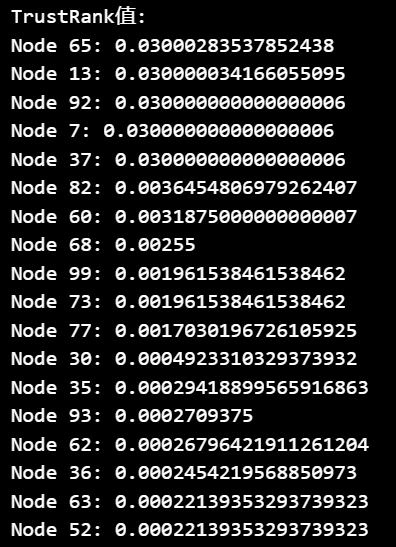
\includegraphics[scale=0.5]{trustrank.png}
		\caption{Part of Trustrank Outcome}
	\end{figure}
	
	\section*{Spam Mass Calculation}
	By utilizing the trust page, pagerank of the spammed graph is calculated, combined with the trustrank, spammass can be calculated:
	$$Spam Mass = \frac{P-T}{P}$$
	where $P$ denotes pagerank, and T denotes trustrank.\\
	Part of Spam Mass outcome is shown below: It is obvious that spam page has heavier spam mass, which means they are more likely to be spam pages.
	\begin{figure}[H]
		\centering
		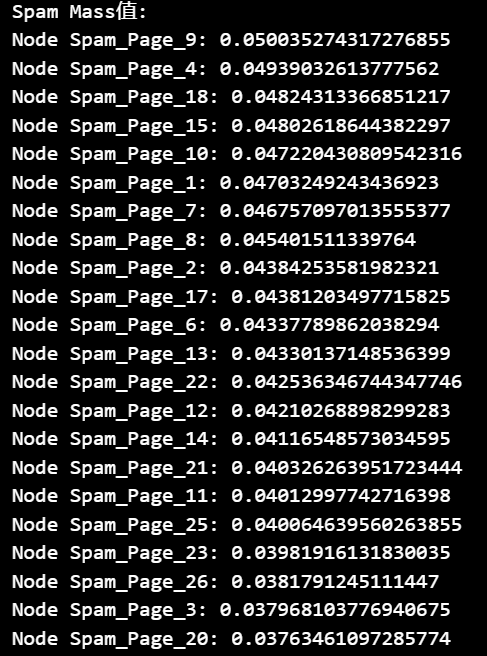
\includegraphics[scale=0.5]{spammass.png}
		\caption{Part of Spam Mass Outcome}
	\end{figure}
	
	\section*{Appendix}
	
	More relevant detailed information you can find in: 
	\href{https://github.com/DingYX0731/Selected-Topics-in-Frontiers-of-Statistics}{\textbf{Github Repository}}
	
	
\end{document}